\section{Introduction}
Particulate matter (PM), or aerosol, is the set of suspended liquid or solid particles found in the atmosphere.
The most relevant to human health are the ones with a diameter smaller than 10 $\mu$m (PM\textsubscript{10})
and smaller than 2.5 $\mu$m (PM\textsubscript{2.5}). With these sizes PM is capable of entering our respiratory
and circulatory system, causing cardiovascular, respiratory and pregnancy problems, and even can increase the
risk of pulmonary cancer and mortality \cite{Mukherjee2017}. PM can also affect visibility, cloud formation
and produce damage to ecosystems and cultural sites \cite{von2015}.\\

The Monterrey Metropolitan Area (MMA) has a severe air pollution problem, with an average annual concentration
of PM higher than the Official Mexican Standard (NOM) in all stations since 2000 \cite{martinez2016}.
The ``Sistema de Monitoreo Ambiental” (SIMA) is the institute that since 1992 reports and shares data on air
pollution over the MMA from its current 13 monitoring stations. According to its 2019 air quality report, more
than half of the year the PM\textsubscript{10} standard is exceeded, so it can be concluded that it is the
main pollutant in the area. The same conclusion that can be reached with the results of Benítez-García \cite{benitez2014} and the National
Institute of Ecology and Climate Change \cite{inecc2011,inecc2019}. Meanwhile, PM\textsubscript{2.5} has data recording problems in most
of the monitoring stations, even though it is known it involves higher health risks. Some of the consequences
of high PM levels are already beginning to be noticed, such as the loss of visibility in the city at certain
times of the day and premature deaths from PM have an average cost of 1\% of the country's gross domestic
product \cite{itdp2019}.\\

Several temporal analyses of PM have been done and also studies trying to pinpoint the sources of this pollutant,
either by chemical characterization and emissions inventories analysis. However, little research has been done
taking into account the Aerosol Optical Depth, that has the advantage of measuring the whole vertical area of
the atmosphere, and not only near the Earth surface. That’s why the aim of this study is to examine PM trends
by comparing PM data measured on ground by SIMA, Aerosol Optical Depth (AOD) estimated by solar irradiance
measurements and AOD data from NASA’s MODIS satellite. We hope to contribute to the better understanding of
the behavior of the pollutant in the complex physiographic zone of the MMA, since it is limited by the Northern
Gulf Coastal Plain in the northeast and the Sierra Madre Oriental in the southwest.\\

\subsection{Study Area}
\begin{figure}[H]
    \centering
    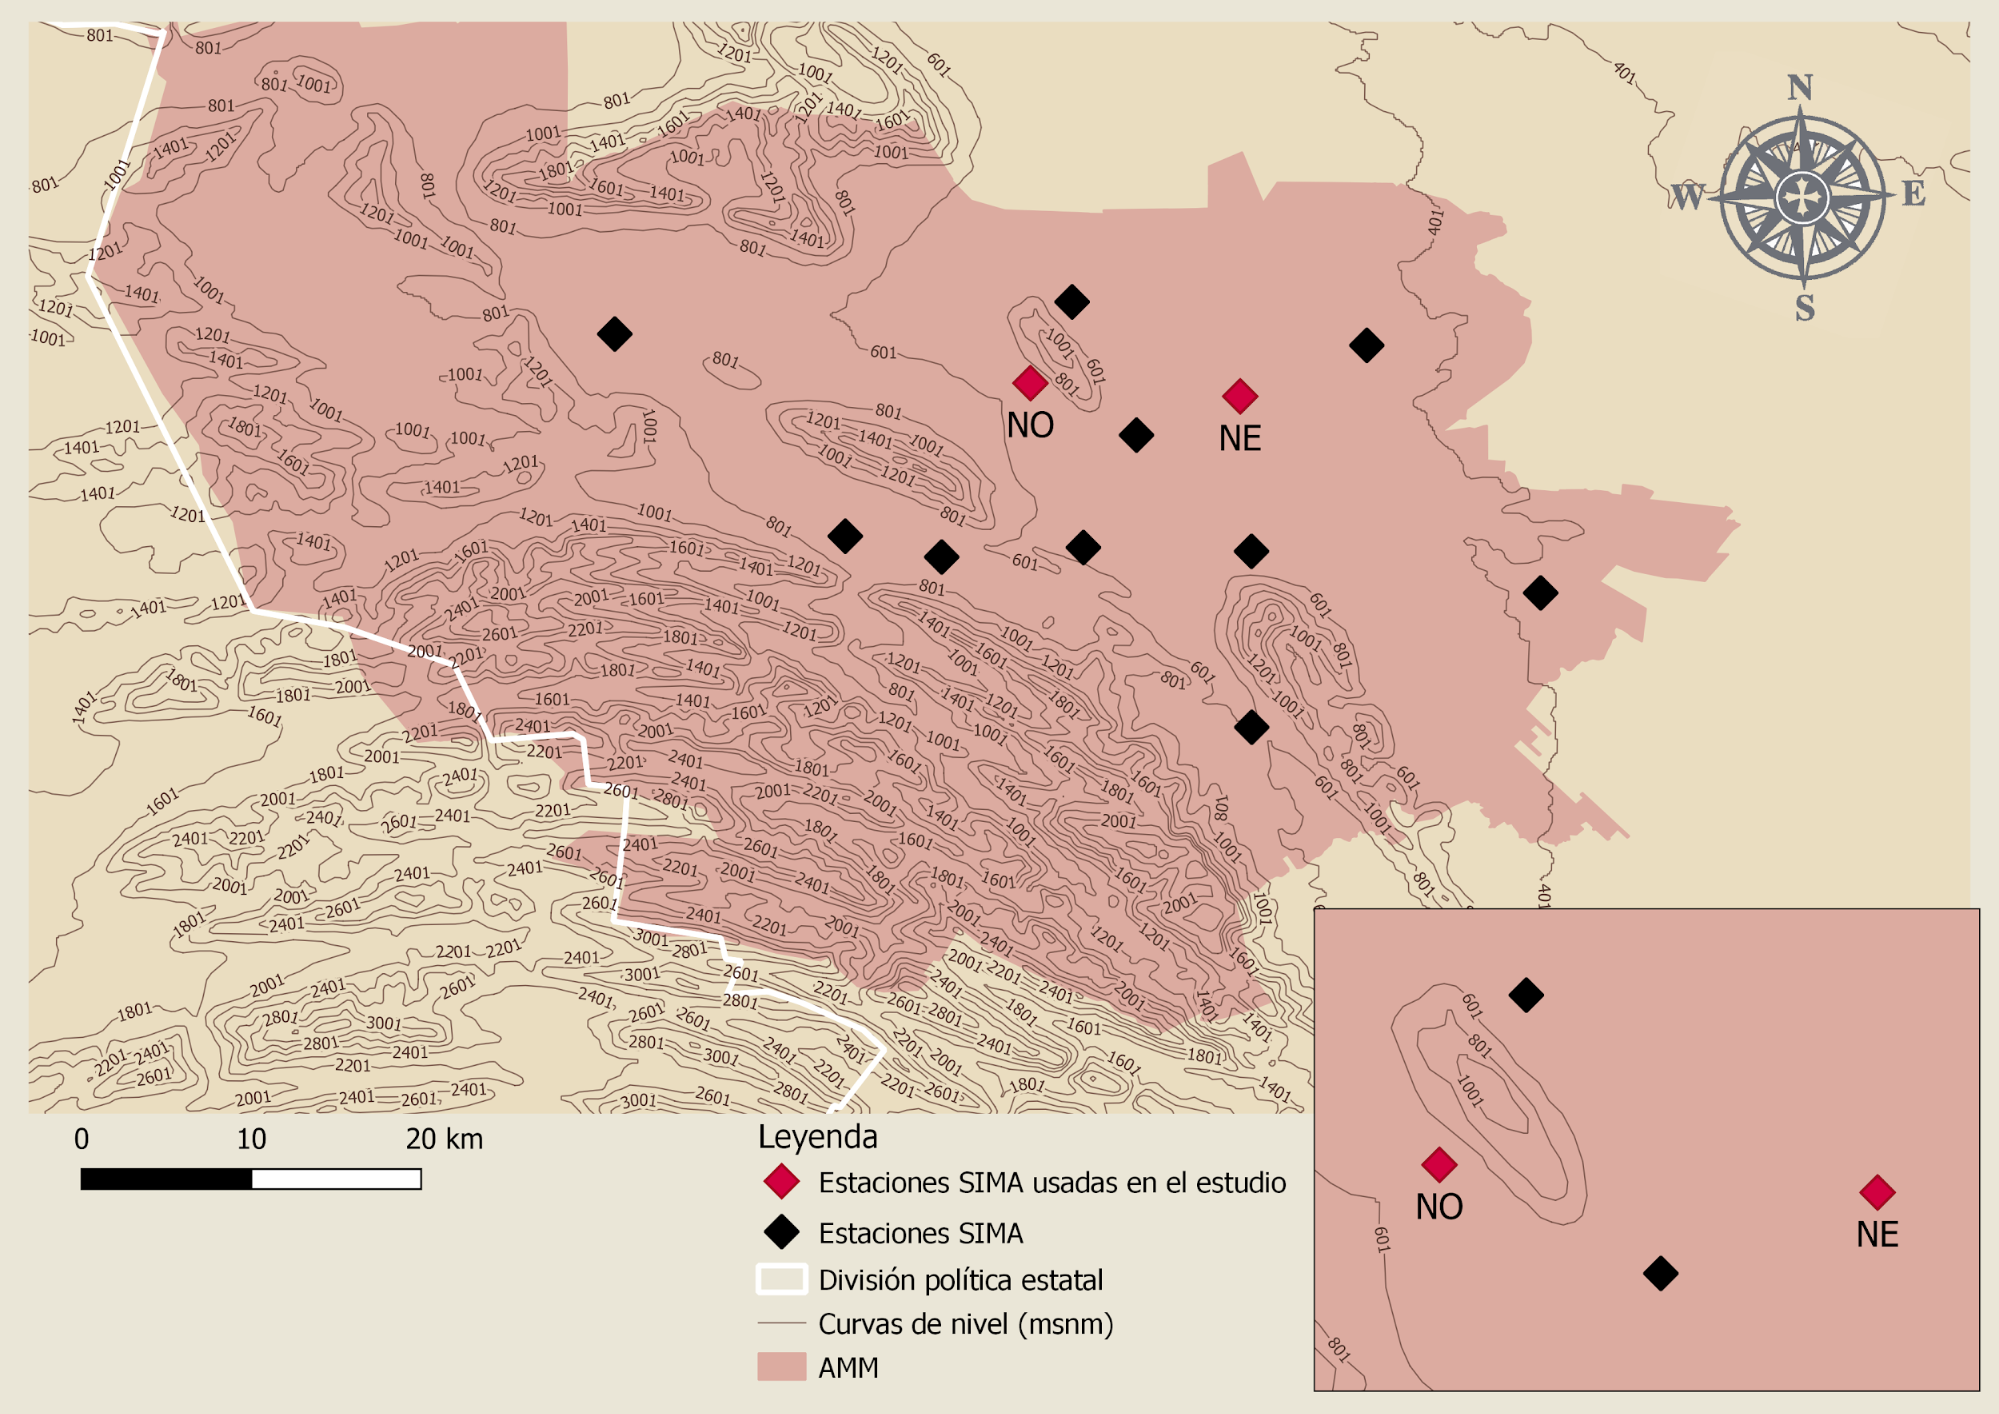
\includegraphics[scale=0.15]{images/map.png}
    \caption{Incluir locación de MMA en México (climas), distribución, estaciones y alturas}
    \label{fig:map}
\end{figure}
The MMA is an industrial power in Northeast Mexico and the third largest urban area in the country.
Given this and the way the urban area developed, the distribution of the PM sources is not homogeneous.
The MMA includes the municipalities of Apodaca, Cadereyta, Escobedo, García, Guadalupe, Juárez, Monterrey,
San Nicolás de los Garza, San Pedro, Santa Catarina and begins to extend towards Santiago with an area of 7,657
km\textsuperscript{2} in 2015 \cite{inegi2015}. They all are limited by the Northern Gulf Coastal Plain
in the northeast and the Sierra Madre Oriental in the southwest, which causes a downward flow of
air from the mountains at night and in the early morning \cite{molina2019}. However, the predominant
direction of the wind is from east to west and this transports the PM to the mountains, which acts as a barrier
by accumulating the particles \cite{gonzalez2011}. A combination of the increase in wind speeds,
high temperatures and humidity, is what makes PM concentrations drop in summer
\cite{gonzalez2011,sima2019}.
